\section*{6. MỘT SỐ BÀI TẬP ỨNG DỤNG HÌNH HỌC CỦA TÍCH PHÂN}

\noindent\textbf{Bài 1.} Các nhà kinh tế sử dụng đường cong Lorenz để minh hoạ sự phân phối thu nhập trong một quốc gia. Gọi $x$ là đại diện cho phần trăm số gia đình trong một quốc gia và $y$ là phần trăm tổng thu nhập. Đường $y = x$ sẽ đại diện cho một quốc gia mà các gia đình có thu nhập như nhau. Đường cong Lorenz $y = f(x)$ biểu thị phân phối thu nhập thực tế. Diện tích hình phẳng giới hạn bởi hai đường này, với $0 \le x \le 100$, biểu thị ``sự bất bình đẳng về thu nhập'' của một quốc gia. Năm $2005$, đường cong Lorenz của Hoa Kỳ có thể được mô hình hoá bởi hàm số
\[
y = \left(0{,}00061x^2 + 0{,}0218x + 1{,}723\right)^2, \quad 0 \le x \le 100,
\]
trong đó $x$ được tính từ các gia đình nghèo nhất đến giàu có nhất (Theo \textit{R. Larson, Brief Calculus: An Applied Approach, 8th edition, Cengage Learning, 2009}).

\noindent\textbf{Lời giải:}

\noindent\textbf{Đáp án:} $297945768{,}18$.

\noindent Sự bất bình đẳng thu nhập của Hoa Kỳ vào năm 2005 là:
\begin{align*}
    &\int_{0}^{100} \left| \left(0{,}00061x^2 + 0{,}0218x + 1723\right)^2 - x \right| \mathrm{d}x \\
    &= \int_{0}^{100} \left| 0{,}00061^2x^4 + 4{,}7524 \cdot 10^{-4} \cdot x^2 + 1723^2 \right. \\
    &\quad \left. + 2{,}6596 \cdot 10^{-5}x^3 + 2{,}10206x^2 + 74{,}1228x \right| \mathrm{d}x \\
    &= \int_{0}^{100} \left( 0{,}00061^2x^4 + 4{,}7524 \cdot 10^{-4} \cdot x^2 + 1723^2 \right. \\
    &\quad \left. + 2{,}6596 \cdot 10^{-5}x^3 + 2{,}10206x^2 + 74{,}1228x \right) \mathrm{d}x \\
    &= \left( 7{,}442 \cdot 10^{-8}x^5 + \frac{11881}{75} \cdot 10^{-6}x^3 + 1723^2x \right. \\
    &\quad \left. + 6{,}649 \cdot 10^{-6}x^4 + \frac{105103}{150000}x^3 + 37{,}0614x^2 \right)\Bigg|_{0}^{100} \\
    &= 7{,}442 \cdot 10^{-8} \cdot 100^5 + \frac{11881}{75} \cdot 10^{-6} \cdot 100^3 + 1723^2 \cdot 100 \\
    &\quad + 6{,}649 \cdot 10^{-6} \cdot 100^4 + \frac{105103}{150000} \cdot 100^3 + 37{,}0614 \cdot 100^2 \\
    &= 297945768{,}18.
\end{align*}

\noindent\textbf{Bài 2.} Khối chỏm cầu có bán kính $R$ và chiều cao $h$ ($0 < h \le R$) sinh ra khi quay hình phẳng giới hạn bởi cung tròn có phương trình $y = \sqrt{R^2 - x^2}$, trục hoành và hai đường thẳng $x = R - h, x = R$ xung quanh trục $Ox$. Tính thể tích của khối chỏm cầu này.

\begin{center}
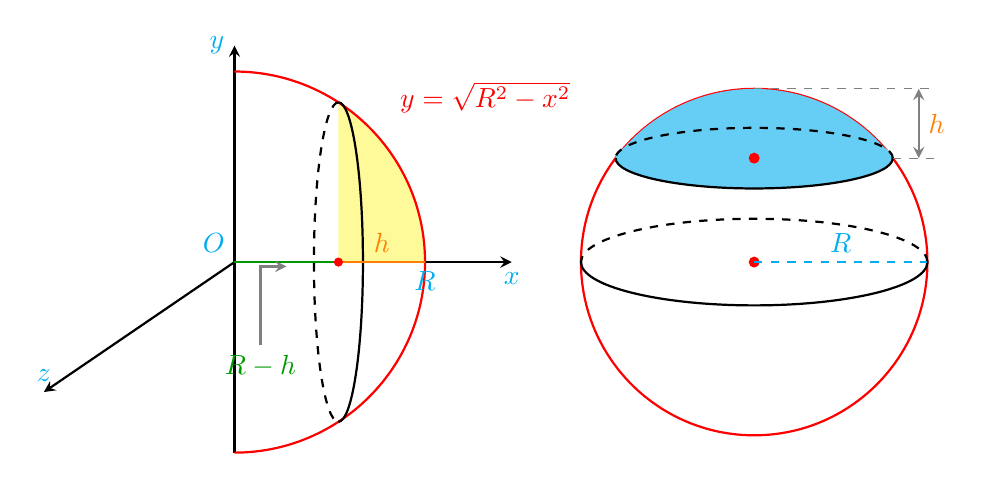
\begin{tikzpicture}[scale=1.1, >=stealth]
    % ==================== HÌNH 1 (BÊN TRÁI) ====================
    \begin{scope}[shift={(0,0)}]
        % Trục tọa độ
        \draw[->, thick] (0,0) -- (3.2,0) node[below, cyan] {$x$};
        \draw[->, thick] (0,-2.2) -- (0,2.5) node[left, cyan] {$y$};
        \draw[->, thick] (0,0) -- (-2.2,-1.5) node[above, cyan] {$z$};
        \node[above left, cyan] at (0,0) {$O$};

        % Miền tô vàng chỏm cầu
        \fill[yellow!40] (1.2,0) -- (1.2,{sqrt(2.2^2 - 1.2^2)}) arc (57.02:0:2.2) -- cycle;

        % Nửa đường tròn bán kính R
        \draw[thick, red] (0,2.2) arc (90:-90:2.2);

        % Mặt cắt elip tại x = R - h: nửa ngoài liền, nửa trong đứt
        \draw[thick] (1.2,{sqrt(2.2^2 - 1.2^2)}) arc (90:-90:0.283 and {sqrt(2.2^2 - 1.2^2)});
        \draw[thick, dashed] (1.2,{sqrt(2.2^2 - 1.2^2)}) arc (90:270:0.283 and {sqrt(2.2^2 - 1.2^2)});

        % Các đoạn thẳng chú thích R-h và h trên trục Ox
        \draw[thick, green!60!black] (0,0) -- (1.2,0);
        \draw[thick, orange] (1.2,0) -- (2.2,0);
        \node[above, orange] at (1.7,0) {$h$};
        \node[below, cyan] at (2.2,0) {$R$};
        
        % Chú thích R - h bằng mũi tên 
        \node[green!60!black] (rh) at (0.3,-1.2) {$R-h$};
        \draw[->, gray, thick] (rh) |- (0.6,-0.05);

        % Điểm đỏ trên trục
        \fill[red] (1.2,0) circle (1.5pt);

        % Nhãn hàm số y = sqrt(R^2 - x^2)
        \node[red, right] at (1.8, 1.9) {$y = \sqrt{R^2 - x^2}$};
    \end{scope}

    % ==================== HÌNH 2 (BÊN PHẢI) ====================
    \begin{scope}[shift={(6,0)}]
        % Khối cầu bên ngoài
        \draw[thick, red] (0,0) circle (2);

        % Đường xích đạo
        \draw[thick] (-2,0) arc (180:360:2 and 0.5);
        \draw[thick, dashed] (2,0) arc (0:180:2 and 0.5);

        % Mặt cắt chỏm cầu màu xanh
        \fill[cyan!60] (0,1.2) ellipse ({sqrt(2^2 - 1.2^2)} and 0.35);
        \fill[cyan!60] ({-sqrt(2^2 - 1.2^2)},1.2) arc (143.13:36.87:2) -- cycle;
        \draw[thick] ({-sqrt(2^2 - 1.2^2)},1.2) arc (180:360:{sqrt(2^2 - 1.2^2)} and 0.35);
        \draw[thick, dashed] ({sqrt(2^2 - 1.2^2)},1.2) arc (0:180:{sqrt(2^2 - 1.2^2)} and 0.35);

        % Các điểm tâm
        \fill[red] (0,0) circle (1.8pt);
        \fill[red] (0,1.2) circle (1.8pt);

        % Bán kính R
        \draw[cyan, dashed, thick] (0,0) -- (2,0);
        \node[cyan, above] at (1,0) {$R$};

        % Đo chiều cao h
        \draw[dashed, gray] (0,2) -- (2.1,2);
        \draw[dashed, gray] ({sqrt(2^2 - 1.2^2)},1.2) -- (2.1,1.2);
        \draw[<->, >=stealth, thick, gray] (1.9,1.2) -- (1.9,2);
        \node[orange, right] at (1.9,1.6) {$h$};
    \end{scope}
\end{tikzpicture}
\end{center}

\noindent\textbf{Lời giải:}

\noindent Thể tích khối chỏm cầu là:
\begin{align*}
    V &= \pi \int_{R-h}^{R} \left(R^2 - x^2\right) \mathrm{d}x \\
    &= \pi \left( R^2x - \frac{x^3}{3} \right)\Bigg|_{R-h}^{R} \\
    &= \pi \left[ R^3 - \frac{R^3}{3} - R^2(R-h) + \frac{(R-h)^3}{3} \right] \\
    &= \pi h^2 \left( R - \frac{h}{3} \right).
\end{align*}

\noindent\textbf{Bài 3.} Cho tam giác vuông $OAB$ có cạnh $OA = a$ nằm trên trục $Ox$ và $\widehat{AOB} = \alpha$ $\left(0 < \alpha \le \dfrac{\pi}{4}\right)$. Gọi $\mathcal{B}$ là khối tròn xoay sinh ra khi quay miền tam giác $OAB$ xung quanh trục $Ox$.
\begin{enumerate}
    \item[a)] Tính thể tích $V$ của $\mathcal{B}$ theo $a$ và $\alpha$.
    \item[b)] Tìm $\alpha$ sao cho thể tích $V$ lớn nhất.
\end{enumerate}

\begin{center}
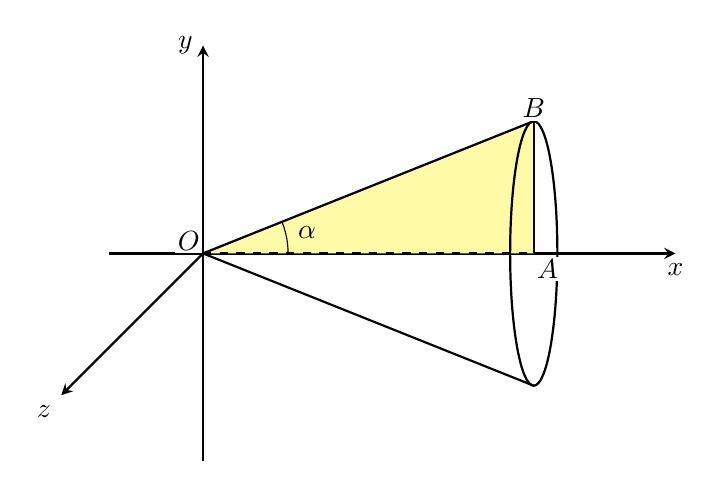
\begin{tikzpicture}[scale=1.2, >=stealth]
    % Hệ trục tọa độ 3 chiều Oxyz
    \draw[->, thick] (-1, 0) -- (5, 0) node[below] {$x$};
    \draw[->, thick] (0, -2.2) -- (0, 2.2) node[left] {$y$};
    \draw[->, thick] (0, 0) -- (-1.5, -1.5) node[below left] {$z$};

    % Các tọa độ điểm
    \coordinate (O) at (0, 0);
    \coordinate (A) at (3.5, 0);
    \coordinate (B) at (3.5, 1.4);

    % Chỉ tô màu vàng đúng phần tam giác OAB ở nửa trên
    \fill[yellow!35] (O) -- (B) -- (A) -- cycle;

    % Vẽ các đường sinh và đường cao
    \draw[dashed, thick] (O) -- (A); 
    \draw[thick] (O) -- (B);       
    \draw[thick] (O) -- (3.5, -1.4); 
    \draw[thick] (A) -- (B);       

    % Đáy hình nón (vẽ hình elip)
    \draw[thick] (3.5, 0) ellipse (0.25cm and 1.4cm);

    % Góc alpha (thu ngắn bán kính lại để không bị nhô ra ngoài)
    \draw (0.9, 0) arc (0:21.8:0.9cm);
    \node at (1.1, 0.22) {$\alpha$};

    % Tên các điểm O, A, B viết rõ ràng
    \node[fill=white, inner sep=1pt] at (O) [above left] {$O$};
    \node[fill=white, inner sep=1pt] at (A) [below right, yshift=-1pt] {$A$};
    \node[fill=white, inner sep=1pt] at (B) [above] {$B$};
\end{tikzpicture}
\end{center}

\noindent\textbf{Lời giải:}

\noindent a) Ta có: $AB = a \tan\alpha$. Khi quay tam giác $AOB$ quanh trục $Ox$ ta được khối nón tròn xoay có bán kính đáy $r = AB = a \tan\alpha$ và chiều cao $h = OA = a$.

\noindent Thể tích khối nón là:
\[
V = \frac{1}{3}\pi r^2 h = \frac{1}{3}\pi \cdot a \cdot a^2\tan^2\alpha = \frac{1}{3}\pi a^3\tan^2\alpha.
\]

\noindent b) Theo a ta có: $V = \frac{1}{3}\pi a^3 \tan^2\alpha$.

\noindent Ta có: $V' = \frac{2}{3}\pi a^3 \tan\alpha \cdot \frac{1}{\cos^2\alpha}$. Với $0 < \alpha \le \dfrac{\pi}{4} \Rightarrow 0 < \tan\alpha < 1$. Do đó, $V' > 0$ nên hàm số $V$ đồng biến trên $\left(0; \dfrac{\pi}{4}\right)$.

\noindent Do đó, $\max\limits_{\left(0;\frac{\pi}{4}\right]} V = V\left(\frac{\pi}{4}\right) = \frac{1}{3}\pi a^3 \tan^2\frac{\pi}{4} = \frac{1}{3}\pi a^3$.

\noindent Vậy giá trị lớn nhất của $V$ là $\dfrac{1}{3}\pi a^3$ khi $\alpha = \dfrac{\pi}{4}$.


\noindent\textbf{Bài 4.} Kiến trúc sư thiết kế một khu sinh hoạt cộng đồng có dạng hình chữ nhật với chiều rộng và chiều dài lần lượt là $60\,\text{m}$ và $80\,\text{m}$. Trong đó, phần được tô màu đậm là sân chơi, phần còn lại để trồng hoa. Mỗi phần trồng hoa có đường biên cong là một phần của parabol với đỉnh thuộc một trục đối xứng của hình chữ nhật và khoảng cách từ đỉnh đó đến trung điểm cạnh tương ứng của hình chữ nhật bằng $20\,\text{m}$ (xem hình minh họa). Diện tích của phần sân chơi là bao nhiêu mét vuông?

\begin{center}
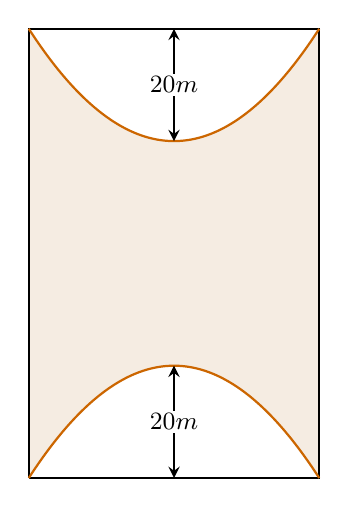
\begin{tikzpicture}
    \begin{axis}[
        xmin=-10, xmax=70,
        ymin=-5, ymax=85,
        axis lines=none,
        samples=100,
        width=6.5cm, height=8cm, % Đã thu nhỏ kích thước lại cho gọn
    ]
        % --- TÔ MÀU PHẦN THÂN CHÍNH Ở GIỮA, ĐỂ TRẮNG 2 ĐẦU PARABOL ---
        \addplot[fill=brown!15, draw=none, domain=0:60] {60 + 0.02222*(x-30)^2} \closedcycle;
        \addplot[fill=white, draw=none, domain=0:60] {20 - 0.02222*(x-30)^2} \closedcycle;

        % --- VẼ VIỀN HÌNH CHỮ NHẬT VÀ ĐƯỜNG CONG PARABOL ---
        \addplot[thick, black] coordinates {(0,0) (60,0) (60,80) (0,80) (0,0)};

        % Đường cong parabol trên và dưới màu cam
        \addplot[thick, orange!80!black, domain=0:60] {60 + 0.02222*(x-30)^2};
        \addplot[thick, orange!80!black, domain=0:60] {20 - 0.02222*(x-30)^2};

        % --- CÁC MŨI TÊN ĐO KHOẢNG CÁCH 20 M KHÍT ---
        \draw[<->, >=stealth, thick] (axis cs:30, 80) -- (axis cs:30, 60);
        \node[fill=white, inner sep=1pt] at (axis cs:30, 70) {\small $20\text{ m}$};

        \draw[<->, >=stealth, thick] (axis cs:30, 20) -- (axis cs:30, 0);
        \node[fill=white, inner sep=1pt] at (axis cs:30, 10) {\small $20\text{ m}$};

    \end{axis}
\end{tikzpicture}
\end{center}

\noindent\textbf{Lời giải:}

\noindent\textbf{Đáp án:} $3200$.

\noindent Đặt hệ trục tọa độ $Oxy$ như hình vẽ.

\begin{center}
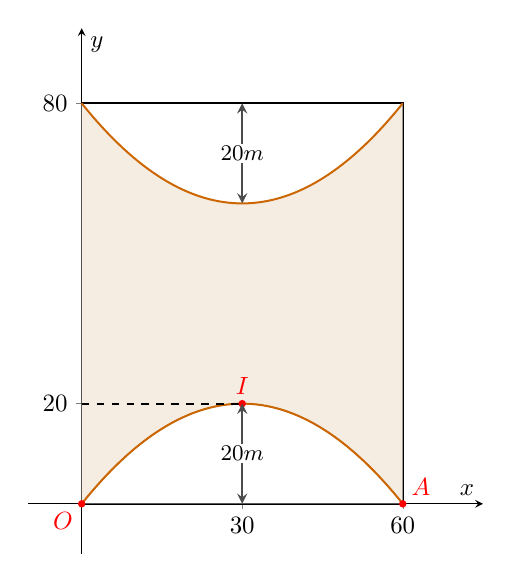
\begin{tikzpicture}[scale=0.9, >=stealth]
    % Sử dụng pgfplots để vẽ hệ trục chuẩn xác
    \begin{axis}[
        xmin=-10, xmax=75,
        ymin=-10, ymax=95,
        axis lines=middle,
        xlabel=$x$, ylabel=$y$,
        xtick={30,60},
        xticklabels={$30$, $60$},
        ytick={20,80},
        yticklabels={$20$, $80$},
        samples=100,
        width=8cm, height=9cm,
    ]
        % Hình chữ nhật tổng thể (chiều rộng 60, chiều cao 80)
        \addplot[thick, black] coordinates {(0,0) (60,0) (60,80) (0,80) (0,0)};
        
        % Tô màu phần sân chơi ở giữa (giới hạn bởi 2 parabol)
        \addplot[fill=brown!15, draw=none, domain=0:60] {80 - (-1/45*x^2 + 4/3*x)} \closedcycle;
        \addplot[fill=white, domain=0:60] {-1/45*x^2 + 4/3*x} \closedcycle;

        % Parabola phía dưới và phía trên
        \addplot[thick, orange!80!black, domain=0:60] {-1/45*x^2 + 4/3*x};
        \addplot[thick, orange!80!black, domain=0:60] {80 - (-1/45*x^2 + 4/3*x)};

        % Đường gióng nét đứt từ điểm I(30; 20) sang trục tung
        \draw[dashed, thick] (axis cs:0,20) -- (axis cs:30,20);
        
        % Các điểm đặc biệt O, I, A
        \fill[red] (axis cs:0,0) circle (1.5pt) node[below left] {$O$};
        \fill[red] (axis cs:30,20) circle (1.5pt) node[above] {$I$};
        \fill[red] (axis cs:60,0) circle (1.5pt) node[above right] {$A$};
        
        % Mũi tên kích thước 20m phía dưới (từ trục x = 0 đến đỉnh parabol y = 20)
        \draw[<->, thick, gray!60!black] (axis cs:30, 0) -- (axis cs:30, 20);
        \node[fill=white, inner sep=1pt] at (axis cs:30, 10) {\small $20\text{ m}$};

        % Mũi tên kích thước 20m phía trên (từ đỉnh parabol y = 60 đến mép trên hình chữ nhật y = 80)
        \draw[<->, thick, gray!60!black] (axis cs:30, 60) -- (axis cs:30, 80);
        \node[fill=white, inner sep=1pt] at (axis cs:30, 70) {\small $20\text{ m}$};
    \end{axis}
\end{tikzpicture}
\end{center}

Nhận thấy hai phần trồng hoa dạng đường parabol có diện tích như nhau. Vậy ta xét đường parabol ở bồn hoa phía dưới có dạng $(P): y = ax^2 + bx + c$ với $a \neq 0$.

Ta có đồ thị $(P)$ đi qua ba điểm là $O(0; 0)$, $I(30; 20)$ và $A(60; 0)$. Thay vào ta thu được hệ phương trình:
\[
\begin{cases}
c = 0 \\
900a + 30b + c = 20 \\
3600a + 60b + c = 0
\end{cases}
\iff
\begin{cases}
a = -\dfrac{1}{45} \\[6pt]
b = \dfrac{4}{3} \\[6pt]
c = 0
\end{cases}
\]

Như vậy, ta có phương trình parabol đó là $y = -\dfrac{1}{45}x^2 + \dfrac{4}{3}x$ và diện tích của phần trồng hoa phía dưới là:
\[
S_{\text{hoa}} = \int_{0}^{60} \left| -\frac{1}{45}x^2 + \frac{4}{3}x \right| \mathrm{d}x = \int_{0}^{60} \left(-\frac{1}{45}x^2 + \frac{4}{3}x\right) \mathrm{d}x = 800 \, (\text{m}^2).
\]

Khi đó, diện tích của phần sân chơi là:
\[
S = 60 \cdot 80 - 2S_{\text{hoa}} = 4800 - 2 \cdot 800 = 3200 \, (\text{m}^2).
\]

\noindent\textbf{Bài 5.} Một vật trang trí có dạng một khối tròn xoay được tạo thành khi quay miền $(R)$ (phần gạch chéo trong hình vẽ) quanh trục $MN$. Biết rằng $ABCD$ là hình chữ nhật với $AB = 6\,\text{cm}, AD = 10\,\text{cm}$ và $M, N$ lần lượt là trung điểm của $AB, CD$. Hai đường cong là đường Elip có hình chữ nhật cơ sở là $ABCD$ và đường tròn tiếp xúc với hai cạnh $AD$ và $BC$ (tham khảo hình vẽ). Tính thể tích của vật trang trí đó (kết quả làm tròn đến hàng phần chục theo đơn vị $\text{cm}^3$).

\begin{center}
\begin{tikzpicture}
    \begin{axis}[
        xmin=-6.5, xmax=6.5,
        ymin=-4.2, ymax=4.2,
        axis lines=none, % Tắt hoàn toàn trục tọa độ
        ticks=none,      % Tắt các vạch chia
        samples=200,
        width=9cm, height=6.5cm,
    ]
        % Hình chữ nhật ABCD cơ sở: x từ -5 đến 5, y từ -3 đến 3
        \addplot[thick, black] coordinates {(-5,3) (5,3) (5,-3) (-5,-3) (-5,3)};
        
        % Nhãn các đỉnh hình chữ nhật A, B, C, D và M, N
        \node at (axis cs:-5, 3.3) [black] {$A$};
        \node at (axis cs:5, 3.3) [black] {$D$};
        \node at (axis cs:-5, -3.3) [black] {$B$};
        \node at (axis cs:5, -3.3) [black] {$C$};
        \node at (axis cs:-5, 0) [left, black] {$M$};
        \node at (axis cs:5, 0) [right, black] {$N$};

        % Gạch chéo toàn bộ phần bên trong hình elip
        \addplot[pattern=north east lines, pattern color=black, draw=none, domain=-5:5] {sqrt(9*(1 - x^2/25))} \closedcycle;
        \addplot[pattern=north east lines, pattern color=black, draw=none, domain=-5:5] {-sqrt(9*(1 - x^2/25))} \closedcycle;

        % Tô nền trắng bên trong hình tròn để che phần gạch chéo ở vùng giữa
        \addplot[fill=white, draw=none, domain=-3:3] {sqrt(9 - x^2)} \closedcycle;
        \addplot[fill=white, draw=none, domain=-3:3] {-sqrt(9 - x^2)} \closedcycle;

        % Vẽ viền đường Elip
        \addplot[thick, black, domain=-5:5] {sqrt(9*(1 - x^2/25))};
        \addplot[thick, black, domain=-5:5] {-sqrt(9*(1 - x^2/25))};
        
        % Vẽ viền đường tròn (C) ở giữa
        \addplot[thick, black, domain=-3:3] {sqrt(9 - x^2)};
        \addplot[thick, black, domain=-3:3] {-sqrt(9 - x^2)};
    \end{axis}
\end{tikzpicture}
\end{center}

\noindent\textbf{Lời giải:}

\noindent\textbf{Đáp án:} $75$.

\begin{center}
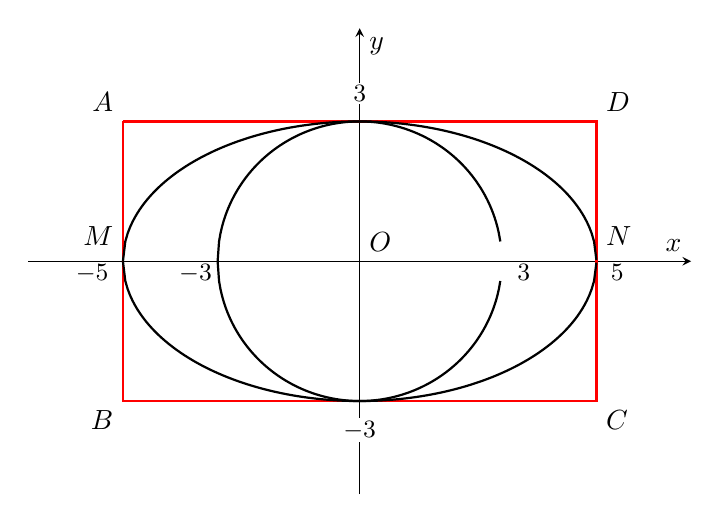
\begin{tikzpicture}
    \begin{axis}[
        xmin=-7, xmax=7,
        ymin=-5, ymax=5,
        axis lines=middle,
        xlabel=$x$, ylabel=$y$,
        xtick=\empty, ytick=\empty, % Tắt tick tự động để chủ động định vị bằng tay
        samples=200,
        width=10cm, height=7.5cm,
    ]
        % Hình chữ nhật ABCD cơ sở (màu đỏ)
        \addplot[thick, red] coordinates {(-5,3) (5,3) (5,-3) (-5,-3) (-5,3)};
        
        % Nhãn các đỉnh hình chữ nhật và điểm M, N, O
        \node at (axis cs:-5, 3) [above left, black] {$A$};
        \node at (axis cs:5, 3) [above right, black] {$D$};
        \node at (axis cs:-5, -3) [below left, black] {$B$};
        \node at (axis cs:5, -3) [below right, black] {$C$};
        \node at (axis cs:-5, 0) [above left, yshift=2pt] {$M$};
        \node at (axis cs:5, 0) [above right, yshift=2pt] {$N$};
        \node at (axis cs:0, 0) [above right] {$O$};

        % --- CÁC MỐC TỌA ĐỘ ĐƯỢC ĐỊNH VỊ THỦ CÔNG KHÔNG CHỒNG LÊN TRỤC VÀ ĐƯỜNG NÉT ---
        % Các số bên trái trục Oy (xích sang trái)
        \node[fill=white, inner sep=1pt, font=\small] at (axis cs:-5, 0) [below left, xshift=-4pt] {$-5$};
        \node[fill=white, inner sep=1pt, font=\small] at (axis cs:-3, 0) [below, xshift=-8pt] {$-3$};
        
        % Các số bên phải trục Oy (xích sang phải)
        \node[fill=white, inner sep=1pt, font=\small] at (axis cs:3, 0) [below, xshift=8pt] {$3$};
        \node[fill=white, inner sep=1pt, font=\small] at (axis cs:5, 0) [below right, xshift=4pt] {$5$};

        % Số 3 phía trên (xích lên cao) và số -3 phía dưới (xích xuống thấp)
        \node[fill=white, inner sep=1pt, font=\small] at (axis cs:0, 3) [above, yshift=6pt] {$3$};
        \node[fill=white, inner sep=1pt, font=\small] at (axis cs:0, -3) [below, yshift=-6pt] {$-3$};
        -------------------------------------------------------------------------------

        % Vẽ viền đường Elip
        \addplot[thick, black, domain=-5:5] {sqrt(9*(1 - x^2/25))};
        \addplot[thick, black, domain=-5:5] {-sqrt(9*(1 - x^2/25))};

        % Vẽ đường tròn tâm O, bán kính R = 3 (liền mạch, không tô màu bên trong)
        \addplot[thick, black, domain=-3:3] {sqrt(9 - x^2)};
        \addplot[thick, black, domain=-3:3] {-sqrt(9 - x^2)};
    \end{axis}
\end{tikzpicture}
\end{center}

\noindent Gắn vào hình chữ nhật $ABCD$ hệ trục tọa độ $Oxy$ với gốc $O$ trùng với giao hai đường chéo, các điểm $M, N$ nằm trên $Ox$ (tham khảo hình vẽ).

\noindent Do $MN$ là trục đối xứng của miền $(R)$ nên khối tròn xoay được tạo thành khi quay miền $(R)$ quanh trục $MN$ trùng với khối tròn xoay được tạo thành khi quay phần $(R)$ nằm phía trên $MN$ quanh $MN$.

\noindent Gọi $V_1, V_2, V$ tương ứng là thể tích của các khối tròn xoay được tạo thành khi quay Elip $(E)$, hình tròn $(C)$ và miền $(R)$ quanh $MN$ (hay quanh $Ox$), ta có $V = V_1 - V_2$.

\noindent Elip $(E)$ có các bán trục $a = \dfrac{1}{2}AD = 5,\, b = \dfrac{1}{2}AB = 3$ nên có phương trình $\dfrac{x^2}{25} + \dfrac{y^2}{9} = 1$.

\noindent Ta có $V_1 = \pi \int_{-5}^{5} 9\left(1 - \frac{x^2}{25}\right) \mathrm{d}x = \pi \left( 9x - \frac{9}{25}x^3 \right)\Bigg|_{-5}^{5} = 60\pi \, (\text{cm}^3)$.

\noindent Hình tròn $(C)$ có tâm tại $O$, bán kính $R = 3$ khi quay quanh $MN$ tạo thành khối cầu tâm $O$, bán kính bằng $3$. Do đó $V_2 = \frac{4}{3}\pi \cdot 3^3 = 36\pi \, (\text{cm}^3)$.

\noindent Thể tích cần tìm là:
\[
V = V_1 - V_2 = 60\pi - 36\pi = 24\pi \approx 75,4 \, (\text{cm}^3) \xrightarrow{\text{làm tròn}} 75.
\]


\noindent\textbf{Bài 6.} Từ hình chữ nhật $ABCD$ có chiều dài $AB = 8\text{ cm}$ và chiều rộng $BC = 4\text{ cm}$, người ta cắt bỏ miền $(R)$ được giới hạn bởi cạnh $CD$ của hình chữ nhật và hai nửa đường thẳng parabol có chung đỉnh là trung điểm cạnh $AB$, chúng lần lượt đi qua hai đầu mút $C, D$ của hình chữ nhật đó (phần tô đậm như hình vẽ). Phần còn lại cho quay quanh trục $AB$ để tạo nên một đồ vật làm trang trí, thể tích của vật trang trí đó bằng bao nhiêu $\text{cm}^3$. Viết kết quả làm tròn đến hàng đơn vị.

\begin{center}
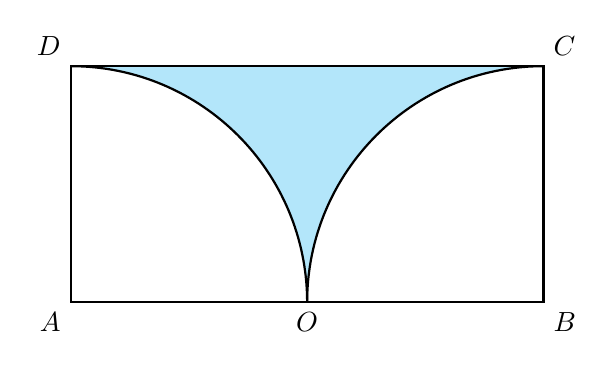
\begin{tikzpicture}[scale=1.5, line width=0.8pt]
    % Định nghĩa các điểm
    \coordinate (A) at (0, 0);
    \coordinate (B) at (4, 0);
    \coordinate (O) at (2, 0);
    \coordinate (C) at (4, 2);
    \coordinate (D) at (0, 2);

    % 1. Tô màu vùng xanh
    % Đi từ D (0,2) sang C (4,2), vòng theo cung CO về O (tâm B(4,0)), rồi vòng theo cung OD về D (tâm A(0,0))
    \fill[cyan!30] (D) -- (C) arc (90:180:2) arc (0:90:2) -- cycle;

    % 2. Vẽ hình chữ nhật ABCD
    \draw (A) -- (B) -- (C) -- (D) -- cycle;

    % 3. Vẽ 2 cung tròn (DO tâm A, CO tâm B)
    \draw (2,0) arc (0:90:2);    % Cung OD (tâm A)
    \draw (2,0) arc (180:90:2);  % Cung OC (tâm B)

    % 4. Nhãn các đỉnh
    \node[below left] at (A) {$A$};
    \node[below right] at (B) {$B$};
    \node[below] at (O) {$O$};
    \node[above right] at (C) {$C$};
    \node[above left] at (D) {$D$};
\end{tikzpicture}
\end{center}
\noindent\textbf{Lời giải}

\noindent \textbf{Trả lời: 201}

\noindent Phương trình Parabol $OC$ có dạng: $y^2 = ax$

\noindent Mặt khác Parabol đi qua điểm $C(4; 4) \Rightarrow 4^2 = 4a \Rightarrow a = 4$

\noindent Khi đó phương trình đường cong $OC$ là $y = \sqrt{4x}$.

\noindent Thể tích của vật thể thu được là: 
$$V = 2\left(\pi \int_{0}^{4} (\sqrt{4x})^2 \,\mathrm{d}x\right) = 64\pi \approx 201\,(\text{cm}^3)$$.
